\section{Combining Time Series and Header Data}

Now that we had fairly good results on Header and Time Series data separately, we wanted to try and see if we could achieve a better performance by using both at once. Given what we've already discussed about random forests being better on larger datasets, we decided to try providing both sets of data to the our ensemble method.

\begin{figure}[h]
\centering
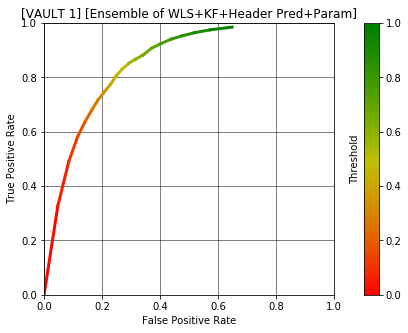
\includegraphics[width=8cm]{body/results/Graphs/Meta+Series/Raw/v1.png}
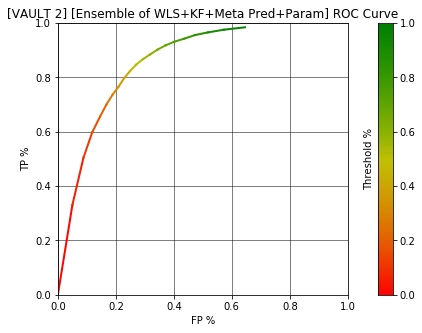
\includegraphics[width=8cm]{body/results/Graphs/Meta+Series/Raw/v2.png}
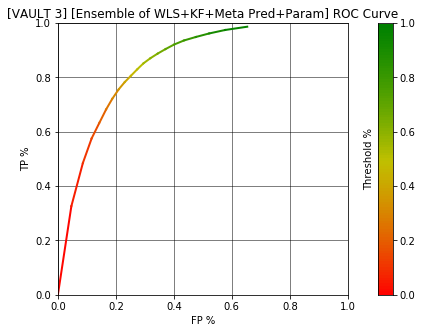
\includegraphics[width=8cm]{body/results/Graphs/Meta+Series/Raw/v3.png}
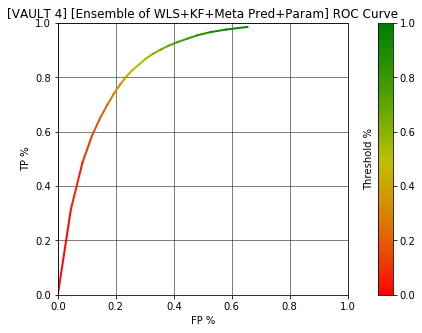
\includegraphics[width=8cm]{body/results/Graphs/Meta+Series/Raw/v4.png}
\caption{ROCs generated based on the ensemble prediction of the outputs of all 15 of our WLS's and KF's (final entries prediction and model parameters) together on the entirety of each validation set and on just ``non-zero'' data. Top Left: Validation set 1. Top Right: Validation set 2. Bottom Left: Validation set 3. Bottom Right: Validation set 4.}
\label{fig:MetSer0}
\end{figure}

Figure \ref{fig:MetSer0} shows the ROCs generated from the predictions of our ensemble when provided with all KF, WLS, and Header information. Comparing these curves with our previous best from Figures \ref{fig:metaonly} and \ref{fig:ensembleTimeCombs} shows that using all available data improves the overall performance. It should be noted, these graphs were made using the full dataset. To see how using only non-zero data performs, we can turn to Figure \ref{fig:MetSern0}.

\pagebreak

\begin{figure}[h]
\centering
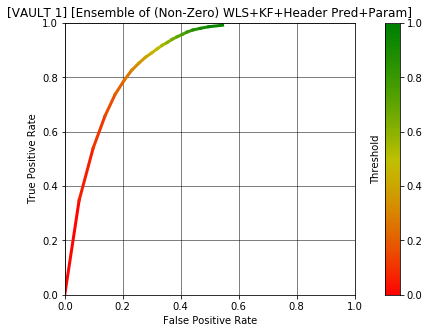
\includegraphics[width=8cm]{body/results/Graphs/Meta+Series/Non-Zero/v1.png}
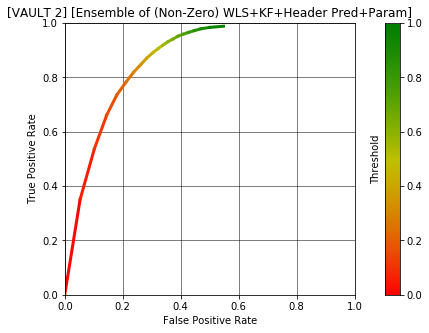
\includegraphics[width=8cm]{body/results/Graphs/Meta+Series/Non-Zero/v2.png}
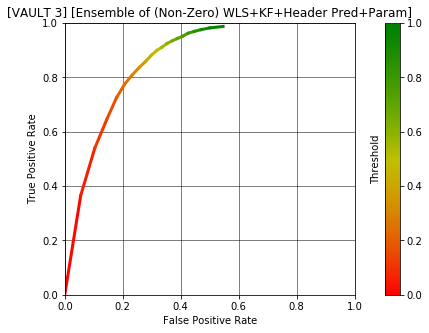
\includegraphics[width=8cm]{body/results/Graphs/Meta+Series/Non-Zero/v3.png}
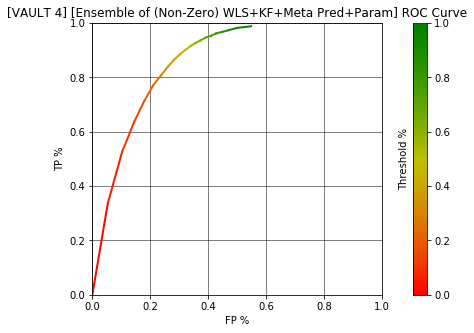
\includegraphics[width=8cm]{body/results/Graphs/Meta+Series/Non-Zero/v4.png}
\caption{ROCs generated based on the ensemble prediction of the outputs of all 15 of our WLS's and KF's (final entries prediction and model parameters) together on the entirety of each validation set and on just ``non-zero'' data. Top Left: Validation set 1. Top Right: Validation set 2. Bottom Left: Validation set 3. Bottom Right: Validation set 4.}
\label{fig:MetSern0}
\end{figure}

Once again, Figure \ref{MetSern0} made using only non-zero data appears to outperform every other method used to this point. A direct comparison of the full ensemble on all data and just non-zero data can be found in Figure \ref{fig:MetSerComp}.

\pagebreak

\begin{figure}[h]
\centering
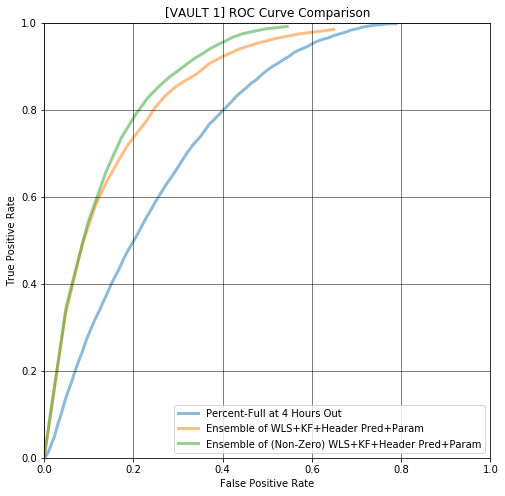
\includegraphics[width=7cm]{body/results/Graphs/Meta+Series/Compare/v1.png}
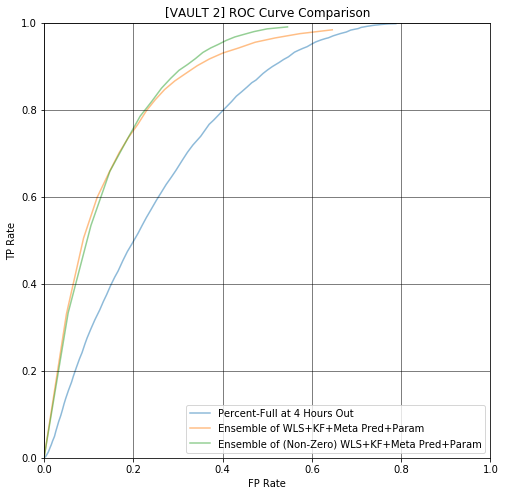
\includegraphics[width=7cm]{body/results/Graphs/Meta+Series/Compare/v2.png}
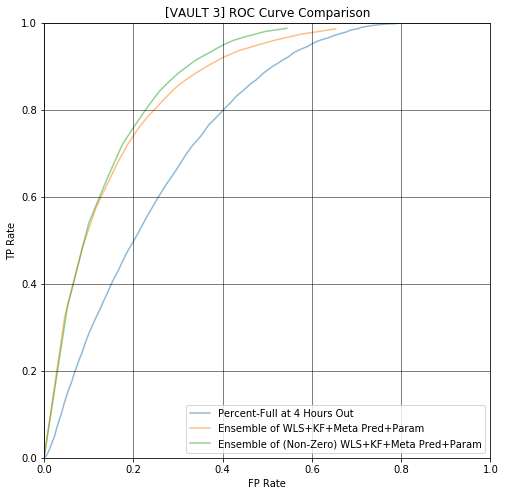
\includegraphics[width=7cm]{body/results/Graphs/Meta+Series/Compare/v3.png}
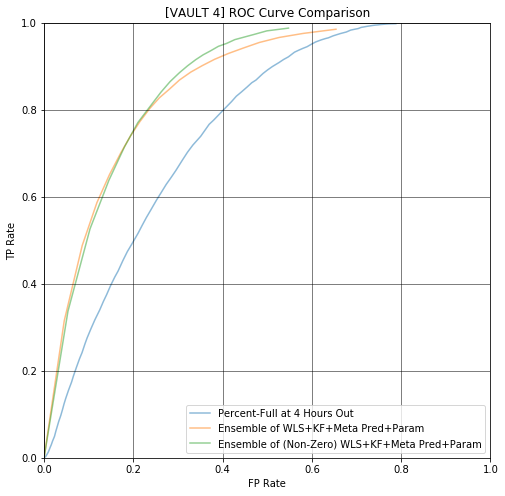
\includegraphics[width=7cm]{body/results/Graphs/Meta+Series/Compare/v4.png}
\caption{ROCs generated based on the ensemble prediction of the outputs of all 15 of our WLS's and KF's (final entries prediction and model parameters) together on the entirety of each validation set and on just ``non-zero'' data. Top Left: Validation set 1. Top Right: Validation set 2. Bottom Left: Validation set 3. Bottom Right: Validation set 4.}
\label{fig:MetSerComp}
\end{figure}

Here we can see that both ensemble methods significantly improve over the baseline. Moreover, using only non-zero data when predicting on an ensemble of all available data appears to perform best overall.

\pagebreak